\chapter{Ausarbeitung}
\section{Aufgabe 1}
Die Zeitreihe der Beschleunigung und Drehraten:\\
\begin{figure}[htpb]\centering
	\subfigure[Beschleunigung]{
		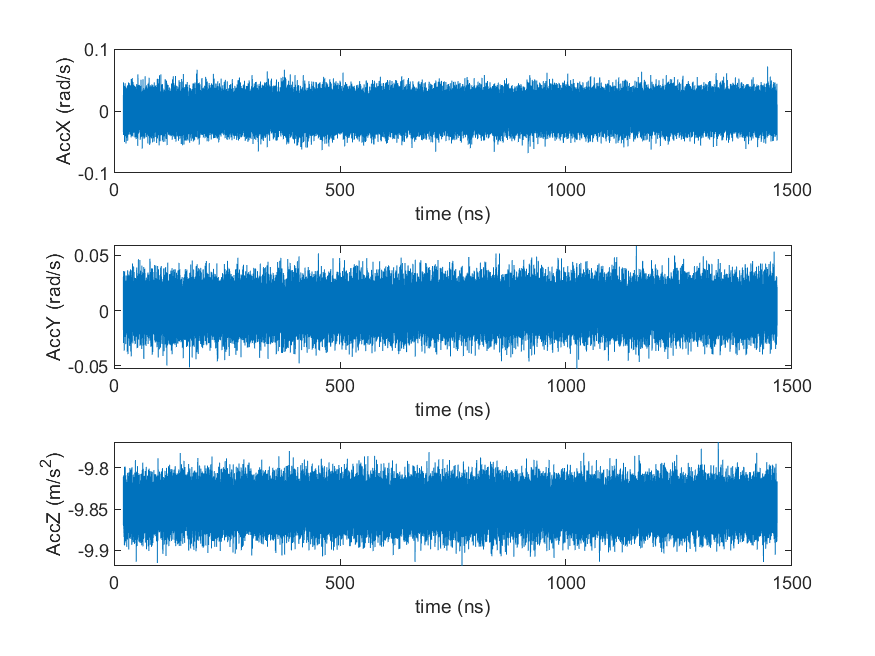
\includegraphics[width=0.9\textwidth]{Beschleunigung.png}}
\end{figure}
\clearpage
\begin{figure}[htpb]\centering
	\subfigure[Drehraten]{
		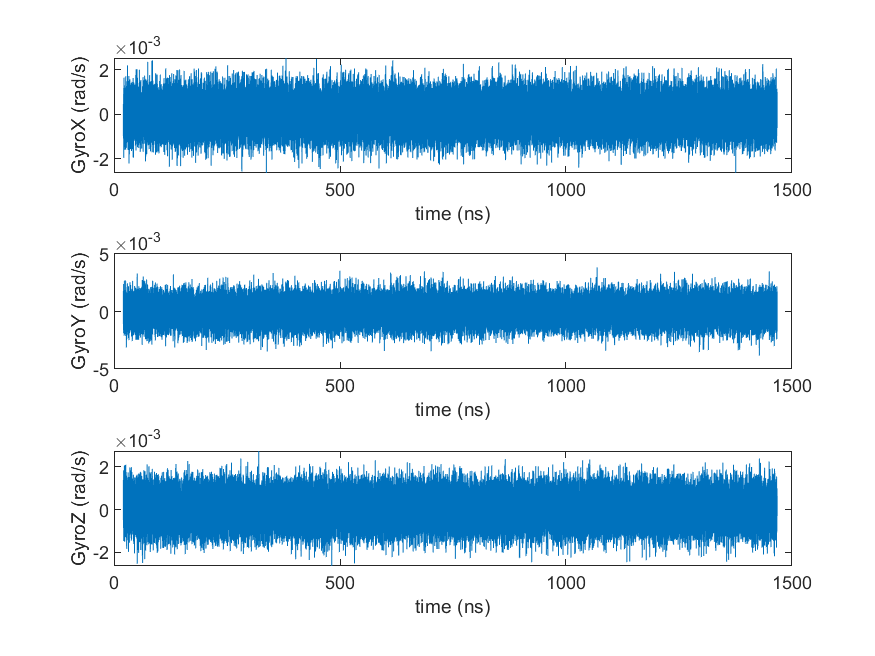
\includegraphics[width=0.9\textwidth]{Gyro.png}}
\end{figure}
Die Standardabweichungen:
\begin{table}[htpb] \centering
	\begin{tabular}{|l|l|}
		\hline
		Messung & Standardabweichung                                 \\ \hline
		accX    & 0.019 $\ut{m/s^2}$ \\ \hline
		accY    & 0.013 $\ut{m/s^2}$                                             \\ \hline
		accZ    & 0.017 $\ut{m/s^2}$                                             \\ \hline
		Yaw     & 6.38e-4  $\ut{rad/s^2}$                                          \\ \hline
		Pitch   & 8.92e-4  $\ut{rad/s^2}$                                             \\ \hline
		Roll    & 6.52e-4  $\ut{rad/s^2}$                                             \\ \hline
	\end{tabular}
\end{table}\\

\clearpage
\section{Aufgabe 2}
Die Orientierungsgleichung wird nummerisch mit Runge-Kutta 3.Ordnung berechnet, Anfangswert ist bekannt. Dann kann man die numeerische Lösung:
\begin{align*}
	\bm{v}^{e}(t_k) = & \hat{\bm{v}}^{e}(t_{k-2}) \\
				+ &[\hat{\bm{C}_p^{e}}(t_{k-2})(3\Delta\bm{v}^{p}(t_{k-1}) - \Delta\bm{v}^{p}(t_k))\\
				+ & \hat{4\bm{C}_p^{e}}(t_{k-1})(\Delta\bm{v}^{p}(t_{k-1}) + \Delta\bm{v}^{p}(t_k))\\
				+ & \hat{\bm{C}_p^{e}}(t_{k})(3\Delta\bm{v}^{p}(t_{k}) - \Delta\bm{v}^{p}(t_k-1))] / 6\\
				- & [2\Omega_{ie}^{e}\hat{\bm{v}}^{e}(t_{k-2}) + \Omega_{ie}^{e}\Omega_{ie}^{e}\hat{\bm{x}}^{e}(t_{k-2})] \cdot \delta t	
\end{align*}
\begin{figure}[htpb]\centering
	\subfigure[Position]{
		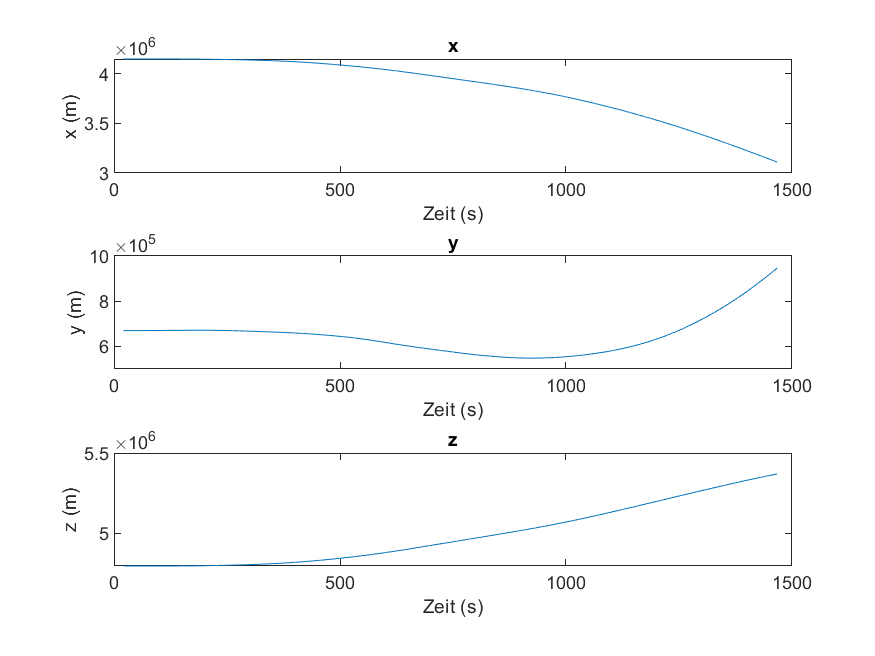
\includegraphics[width=0.8\textwidth]{A2_pos.png}}
\end{figure}
\begin{figure}[htpb]\centering
	\subfigure[Geschwindigkeit]{
		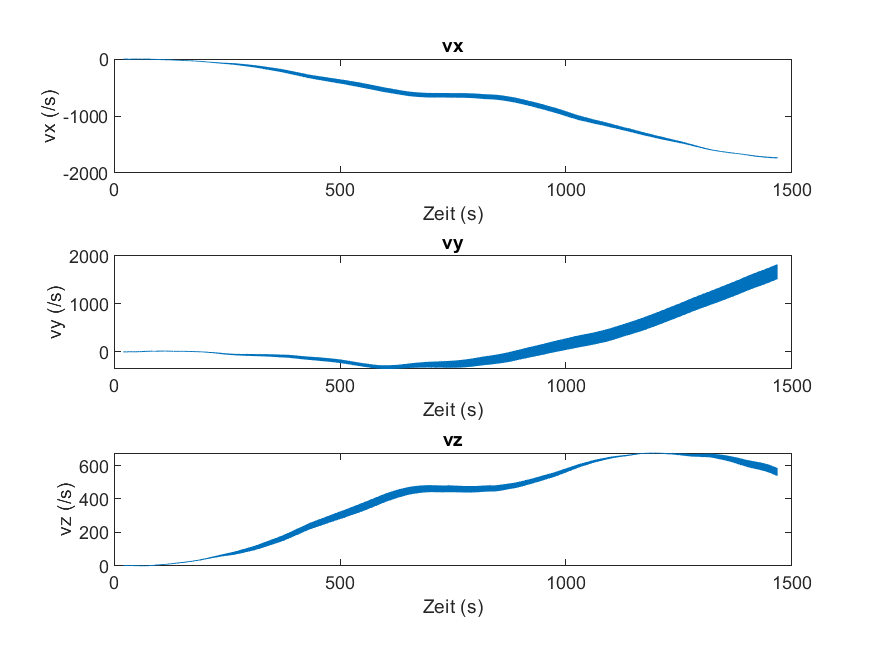
\includegraphics[width=0.8\textwidth]{A2_vel.png}}
\end{figure}
\begin{figure}[htpb]\centering
	\subfigure[Euler Winkel der DCM]{
		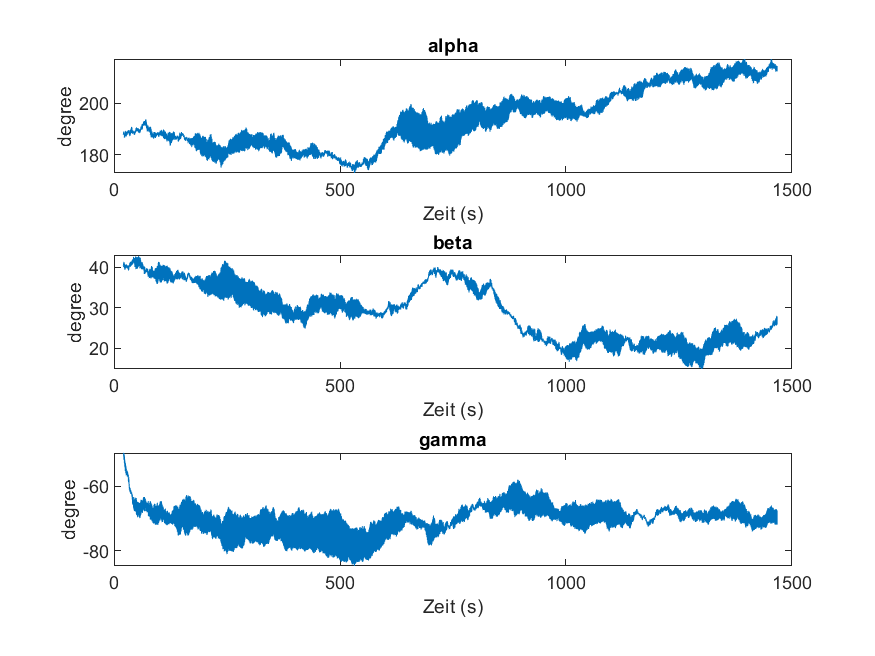
\includegraphics[width=0.8\textwidth]{A2_euler.png}}
\end{figure}\\
Dle Geschwindigkeit und Orientierung sind mit große Schwingungen. Die Änderungen sind am Anfang klein und nach einigen Minuten Größe. Die Position sind schnell von richtigen Werte abweichend.
\clearpage
\section{Aufgabe 3}
Die wahre Position ist $48.78070719 \ut{N}$, $9.17158708 \ut{E}$, $326.568 \ut{m}$, Die Wahre Geschwindigkeit ist $\bm{0}$, Die vorwärts integriete Navigationslösung wird mit KF korrigiert. \\\\
Die Positionen, die berechnet jeweils mit Update Schritt 5 s,60 s und 120 s sind, liegt in \autoref{fig:positionen}.
\begin{figure}[htpb]\centering
	\subfigure[5s]{
		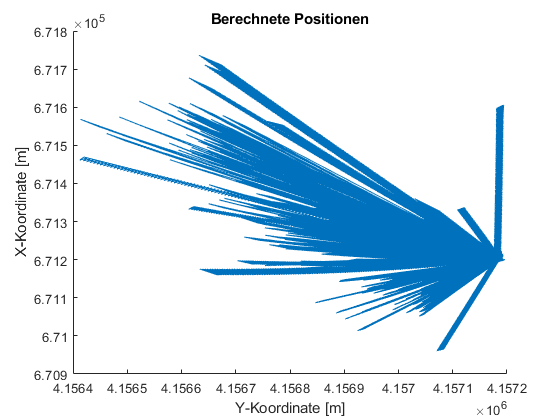
\includegraphics[width=0.45\textwidth]{A3_5_tra.png}}
	\subfigure[60s]{
		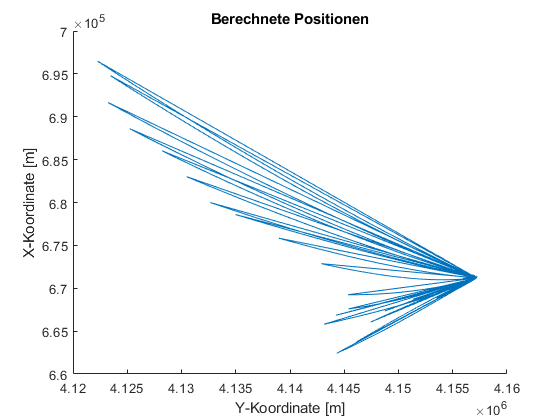
\includegraphics[width=0.45\textwidth]{A3_60_tra.png}}
	\subfigure[120s]{
		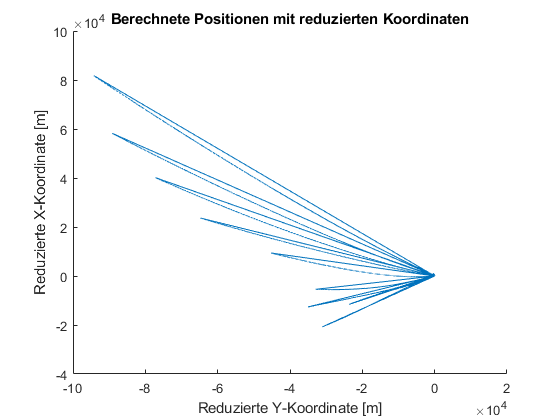
\includegraphics[width=0.45\textwidth]{A3_120_tra.png}}
	\caption{Positionen}
	\label{fig:positionen}
\end{figure}\\
Die Positionsabweichung von wahrer Position liegt in \autoref{fig:abweichung}, je häufiger die Update war, desto sind die Abweichungen deutlich kleiner. 
\begin{figure}[htpb]\centering
	\subfigure[5s]{
		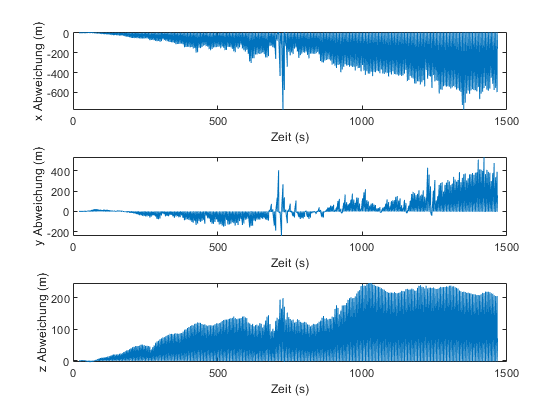
\includegraphics[width=0.45\textwidth]{A3_5_ab.png}}
	\subfigure[60s]{
		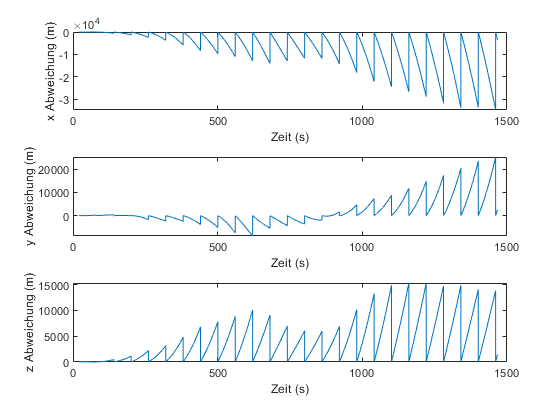
\includegraphics[width=0.45\textwidth]{A3_60_ab.png}}
	\subfigure[120s]{
		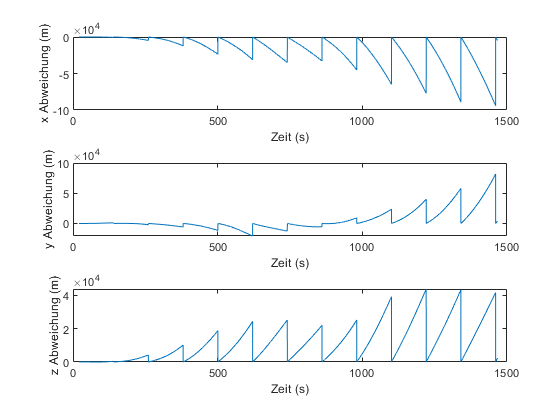
\includegraphics[width=0.45\textwidth]{A3_120_ab.png}}
	\caption{Positionen Abweichungen}
	\label{fig:abweichung}
\end{figure}\\\\
Die Varianz von Position und Geschwindigkeit werden nach der Korrektur durch den Kf geringer.\autoref{fig:Varianz}
\begin{figure}[htpb]\centering
	\subfigure[5s]{
		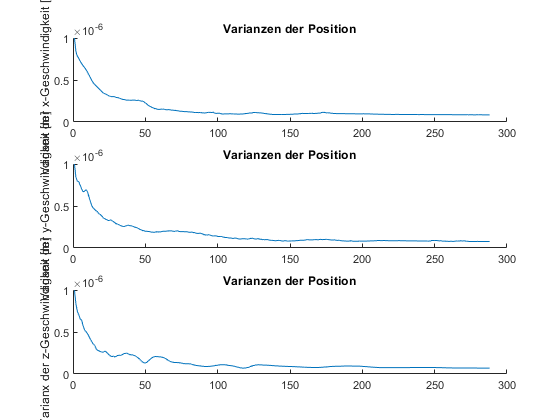
\includegraphics[width=0.45\textwidth]{A3_5_posvar.png}}
	\subfigure[5s]{
		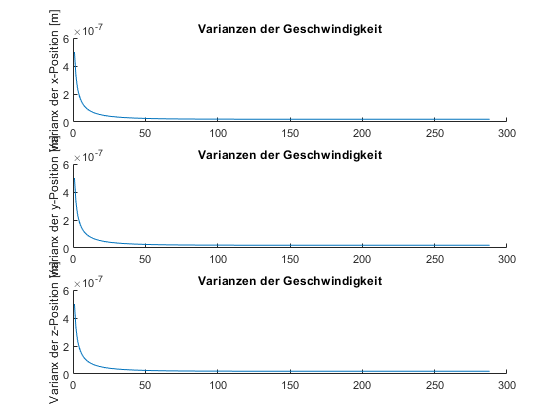
\includegraphics[width=0.45\textwidth]{A3_5_velvar.png}}
	\subfigure[60s]{
		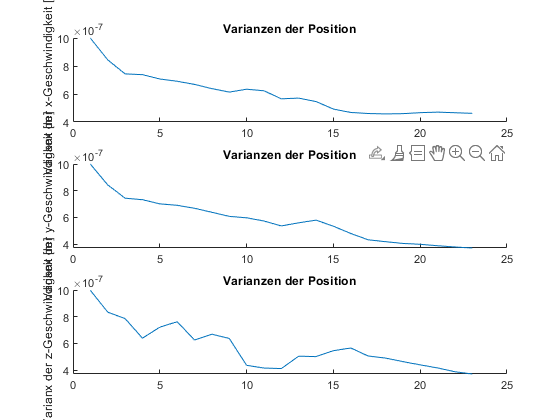
\includegraphics[width=0.45\textwidth]{A3_60_posvar.png}}
	\subfigure[60s]{
		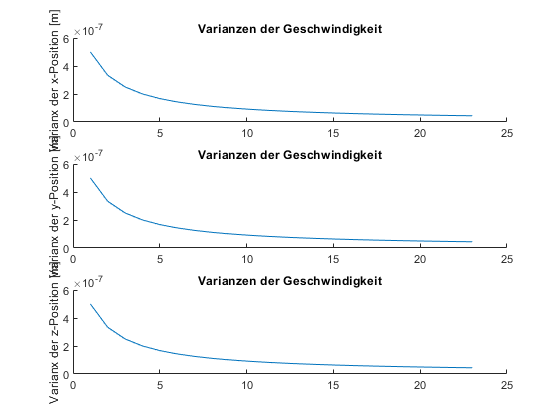
\includegraphics[width=0.45\textwidth]{A3_60_velvar.png}}
	\subfigure[120s]{
		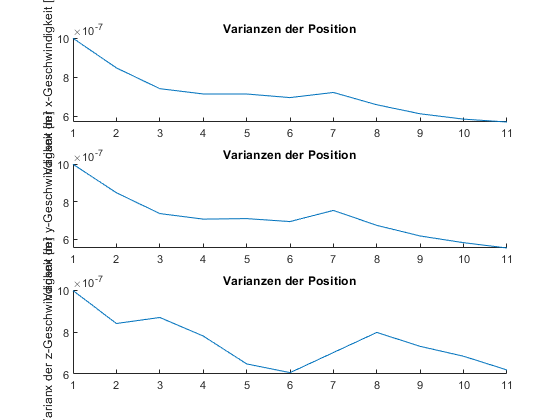
\includegraphics[width=0.45\textwidth]{A3_120_posvar.png}}
	\subfigure[120s]{
		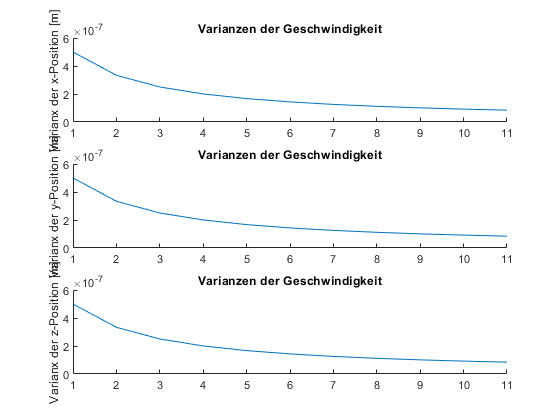
\includegraphics[width=0.45\textwidth]{A3_120_velvar.png}}
	\caption{Varianz}
	\label{fig:Varianz}
\end{figure}